% PLANTILLA APA7
% Creado por: Isaac Palma Medina
% Última actualización: 25/07/2021
% @COPYLEFT

% Fuentes consultadas (todos los derechos reservados):  
% Normas APA. (2019). Guía Normas APA. https://normas-apa.org/wp-content/uploads/Guia-Normas-APA-7ma-edicion.pdf
% Tecnológico de Costa Rica [Richmond]. (2020, 16 abril). LaTeX desde cero con Overleaf (1 de 3) [Vídeo]. YouTube. https://www.youtube.com/watch?v=kM1KvHVuaTY Weiss, D. (2021). 
% Formatting documents in APA style (7th Edition) with the apa7 LATEX class. https://ctan.math.washington.edu/tex-archive/macros/latex/contrib/apa7/apa7.pdf @COPYLEFT

%+-+-+-+-++-+-+-+-+-+-+-+-+-++-+-+-+-+-+-+-+-+-+-+-+-+-+-+-+-+-++-+-+-+-+-+-+-+-+-+

% Preámbulo
\documentclass[stu, 12pt, letterpaper, donotrepeattitle, floatsintext, natbib, helv]{apa7}
\usepackage[utf8]{inputenc}
\usepackage{comment}
\usepackage{marvosym}
\usepackage{graphicx}
\usepackage{float}
\usepackage[normalem]{ulem}
\usepackage[spanish]{babel} 
%\usepackage{titling}
\let\apasubparagraph\subparagraph
\let\subparagraph\paragraph
\usepackage[compact]{titlesec}
\let\subparagraph\apasubparagraph
\usepackage{hyperref}
\selectlanguage{spanish}
\useunder{\uline}{\ul}{}
\newcommand{\myparagraph}[1]{\paragraph{#1}\mbox{}\\}
\graphicspath{{./Images/}}
\titleformat{\section}{\normalfont\large\bfseries}{\thetitle. \quad }{0pt}{}[{ \titlerule[0.8pt]}]
\titleformat{\subsection}{\normalfont\bfseries}{}{}{}[]

% Portada

\begin{document}
\begin{titlepage}
    \centering
    \vfill
    \LARGE Tarea \#2\\
    \vskip2cm
    \large Diego Quirós Artiñano \\
    Universidad Nacional de Costa Rica \\
    EIF-202: Soporte Técnico \\ 
    Carolina Gómez Fernández \\
    03 de abril, 2022 \\
    \vfill
    
\includegraphics[width = 0.4\textwidth]{/home/xarthy/UNAImage/UNA.png} \\
    \vfill
    \vfill
    % (autores separados, consultar al docente)
    % Manera oficial de colocar los autores:
    %\author{Autor(a) I, Autor(a) II, Autor(a) III, Autor(a) X}
\end{titlepage}

% Índices
\pagenumbering{roman}
    % Contenido
\renewcommand\contentsname{\largeÍndice}
\tableofcontents
\setcounter{tocdepth}{2}
\newpage
    % Figuras
\renewcommand{\listfigurename}{\largeÍndice de fíguras}
\listoffigures
\newpage
    % Tablas
\renewcommand{\listtablename}{\largeÍndice de tablas}
\listoftables
\newpage

% Cuerpo
\pagenumbering{arabic}

%------------------------------------------------------------------------------------
\section{Introducción}
En esta tarea se va a investigar sobre dos componentes, generar circuitos con los dos y resolver problemas de circuitos (resistencias, voltajes y corrientes) implementando lo aprendido en clase de resistencias en serie y en paralelas.

%------------------------------------------------------------------------------------
\section{Investigar el uso del temporizador 555 y de la fotorresistencia}
Para esta sección investigué sobre las fotorresistencias, según Dynamo Electronics(\cite{fotorresistencia}), la fotorresistencia sirve como una resistencia normal, pero es afectada por la luz, entre más luz haya, menos resistencia, entonces más voltaje pasa.
Al investigar sobre el temporizador, primero tenía que ver lo que era en Tinkercad, porque lo tengo configurado en inglés, ahí me percate que en inglés se llama Timer 555. Ya con esto entonces tengo mejor idea de lo que hace el aparato, osea sirve para mandar pulsos en un tiempo determinado. Para continuar con la investigación, según Electronics Tutorials (\cite{temporizadorDef}), el nombre viene de que internamente trae tres $5k\Omega$, se generan dos comparadores, se utiliza para generar pulsos singulares, o largos tiempos de espera. 

%----------------------------------------------------------------------------------------------------------------------------------
\section{Realizar un circuito utilizando el temporizador 555 o la fotorresistencia}
\begin{figure}[H]
    \centering
    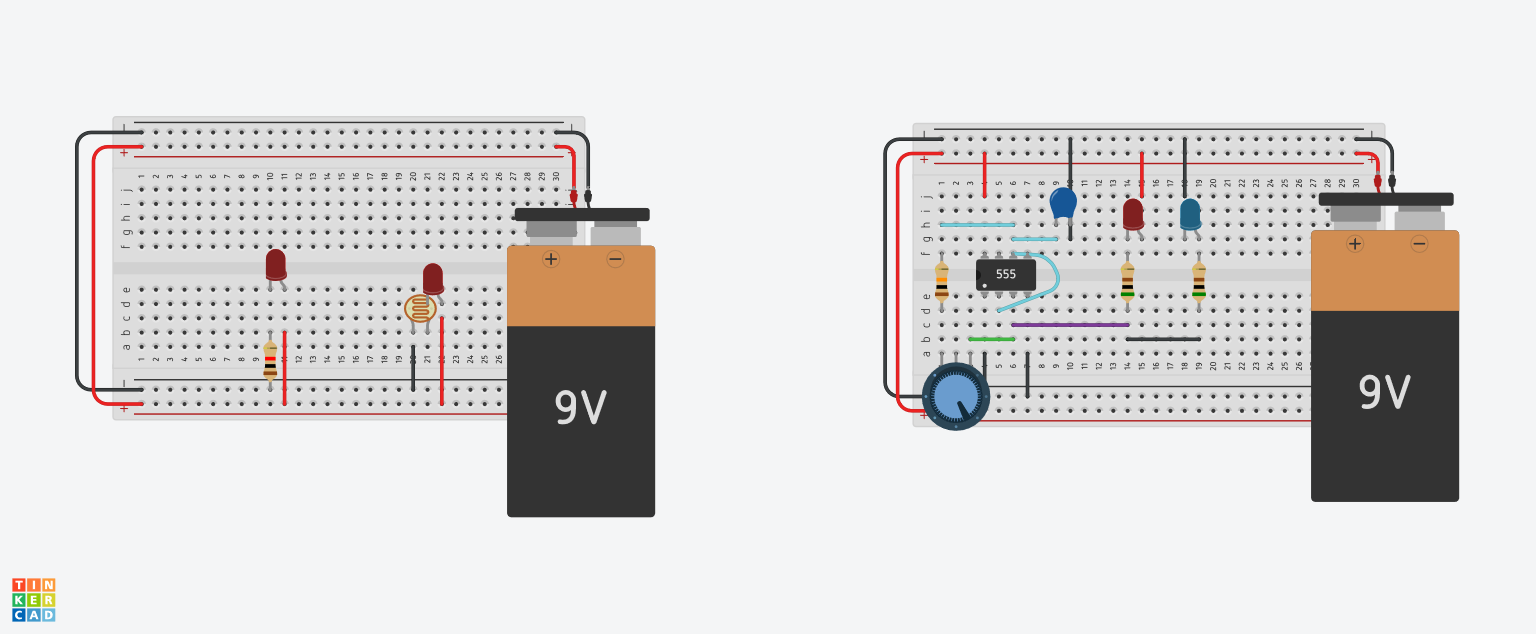
\includegraphics[width=1\textwidth]{Circuits.png}
    \caption{Circuitos de fotorresistencia y temporizador 555}
    \label{fig:figureTinkercad}
\end{figure}

\noindent\cite{tinkercad}
Para esta sección generé dos circuitos, el de la izquierda es de la fotorresistencia, como sirve como una resistencia normal, solo que afectada por la luz lo puse a la par de una resistencia normal para ver la diferencia.
El de la derecha es el circuito del temporizador 555, usé un video de Rosie Research \cite{videoTemporizador}, para ver como se conectaba el temporizador 555, con esto generé las luces de policía que hace en el video y aprendí que no solo se puede conectar con el potenciómetro, sino que se necesita un capacitador para usarlo de manera \textit{"Flip-Flop"} (Que intercambia el led que utiliza, como es un timer entonces continuamente está cambiando de led).
%----------------------------------------------------------------------------------------------------------------------------------------------------------------------
\section{Obtener los siguientes datos de la figura 2}
\begin{itemize}
    \item Resistencia total
    \item Corriente total
    \item Voltaje en cada resistencia
    \item Intensidad en cada resistencia
\end{itemize}
\begin{figure} [H]
    \centering
    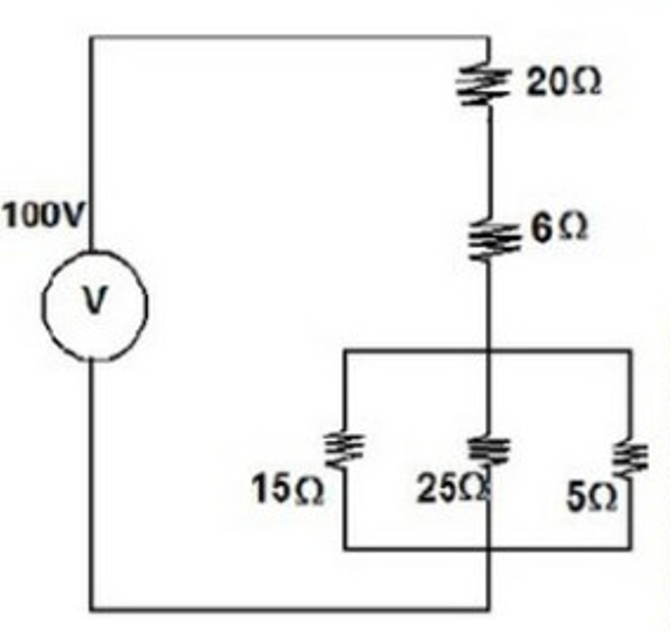
\includegraphics[width=0.4\textwidth] {Problem3.png}
    \caption{Problema 3}
    \label{fig:figureP3}
\end{figure}
\subsection{Resistencia total:}
\[R_T = 20\Omega + 6\Omega + (\frac{1}{15\Omega} + \frac{1}{25\Omega} + \frac{1}{5\Omega})\]
\[R_T = 26 + (\frac{5}{75} + \frac{3}{75} + \frac{15}{75})\]
\[R_T = 26 + \frac{23}{75}\]
\[R_T = 26 + 3.26\]
\[R_T = 29.26\Omega\]
\subsection{Corriente total:}
\[I_T = \frac{V_T}{R_T}\]
\[I_T = \frac{100V}{29.26\Omega}\]
\[I_T = 3.42A\]
\subsection{Voltaje en cada resistencia:}
\[V_1 = R_1 * I_T\]
\[V_1 = 20 * 3.42\]
\[V_1 = 68.4V\]
\[V_2 = R_2 * I_T\]
\[V_2 = 6 * 3.42\]
\[V_2 = 20.52V\]
\[V_3 = V_4 = V_5 = V_T - V_1 - V_2\]
\[V_3 = V_4 = V_5 = 11.02V\]


\subsection{Intensidad en cada resistencia:}
\[I_1 = I_2 = \frac{V_T}{R_T}\]
\[I_1 = \frac{100}{29.26}\]
\[I_1 = 3.42A\]
\[I_3 = \frac{V_3}{R_3}\]
\[I_3 = \frac{11.02}{15}\]
\[I_3 = 0.73\]
\[I_4 = \frac{V_4}{R_4}\]
\[I_4 = \frac{11.02}{25}\]
\[I_4 = 0.44\]
\[I_5 = \frac{V_5}{R_5}\]
\[I_5 = \frac{11.02}{5}\]
\[I_5 = 2.20\]
Nota: \[I_3 + I_4 + I_5 = 3.37 \neq 3.42\] no es exacto por redondeos.
%----------------------------------------------------------------------------------------------------------------------------------------------------------------------
\section{En el circuito de la figura, calcular la resistencia total y la resistencia R3}
\begin{figure}[H]
    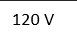
\includegraphics[width=0.2\textwidth]{Problem4-1.png}
    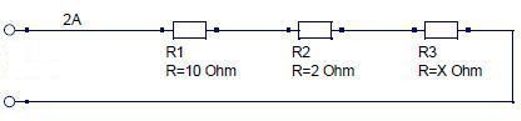
\includegraphics[width=0.9\textwidth]{Problem4-2.png}
    \caption{Problema 4}
    \label{fig:figureP4}
\end{figure}

\[R_T = \frac{V_T}{I_T}\]
\[R_T = \frac{120}{2}\]
\[R_T = 60\Omega\]
\[R_3 = R_T - R_1 - R_2\]
\[R_3 = 60 - 10 - 2\]
\[R_3 = 48\Omega\]
%----------------------------------------------------------------------------------------------------------------------------------------------------------------------

\section{Cinco resistencia idénticas se montan en paralelo sobre una línea de 100V. Calcular la intensidad que pasa por el grupo sabiendo que la resistencia de cada lámpara vale 400 ohmios.}
\begin{figure}[H]
    \centering
    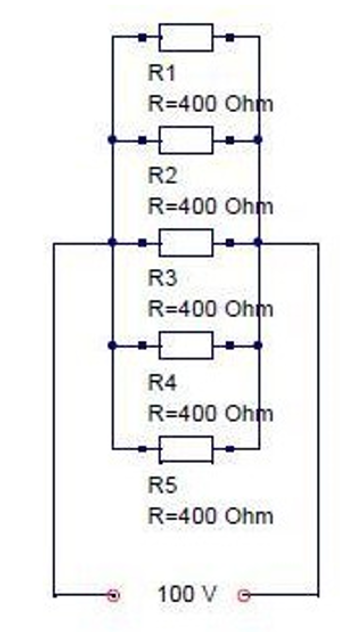
\includegraphics[width=0.4\textwidth]{Problem5.png}
    \caption{Problema 5}
    \label{fig:figureP5}
\end{figure}

\[\frac{1}{R_T} = \frac{1}{R_1} + \frac{1}{R_2} + \frac{1}{R_3} + \frac{1}{R_4} + \frac{1}{R_5}\]
\[\frac{1}{R_T} = \frac{1}{400} + \frac{1}{400} + \frac{1}{400} + \frac{1}{400} + \frac{1}{400}\]
\[\frac{1}{R_T} = \frac{5}{400}\]
\[R_T = \frac{400}{5}\]
\[R_T = 90\Omega\]

\[I_T = \frac{V_T}{R_T}\]
\[I_T = \frac{100}{90}\]
\[I_T = 1.11A\]
%----------------------------------------------------------------------------------------------------------------------------------------------------------------------
\section{Conclusión}
En este documento se aumentó el conocimiento sobre los componentes de circuitos, específicamente la fotorresistencia y el temporizador 555, también se resolvieron problemas de resistencias, voltajes y corrientes en series y paralelas.

\newpage
% Referencias
\renewcommand\refname{\large\textbf{Referencias}}
\bibliography{ref}

\end{document}